\chapter{Литералы в Haskell}

\section{Виды литералов}

В Хаскель можно выделить три вида литералов: целочисленные, вещественные,
символьные и строковые.

\begin{figure}[H]
\label{bool}
\begin{lstlisting}[language=Haskell]
data Bool = True | False
\end{lstlisting}
\caption{Определение значений True и False}
\end{figure}

В отличие от многих других языков, логические значения \texttt{True} и
\texttt{False} являются идентификаторами. Они входят в состав стандартного
модуля \texttt{Prelude} и определены как показано в листинге \ref{bool}.

\begin{figure}[H]
\centering
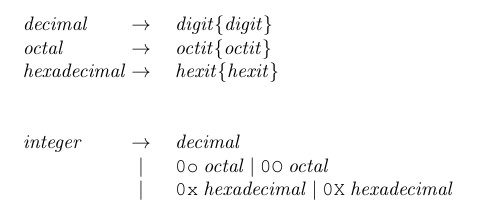
\includegraphics[scale=0.66]{pic-integral-literals}
\caption{Лексическая структура целочисленных литералов}
\end{figure}

Целочисленные литералы представляют значения натуральных чисел, включая ноль.
Существует синтаксис для записи в различных системах счисления: десятичной,
восьмеричной, шестнадцатеричной. Примеры: \texttt{30}, \texttt{0o36},
\texttt{0O36}, \texttt{0x1E}, \texttt{0X1E}.

\begin{figure}[H]
\centering
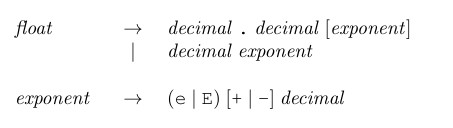
\includegraphics[scale=0.66]{pic-rational-literals}
\caption{Лексическая структура вещественных литералов}
\end{figure}

Вещественные литералы представляют рациональные числа. Можно использовать как
обычные десятичные дроби, так и научную форму записи с указанием мантиссы и
порядка. Примеры: \texttt{123.456}, \texttt{0.123456e3}.

\begin{figure}[H]
\centering
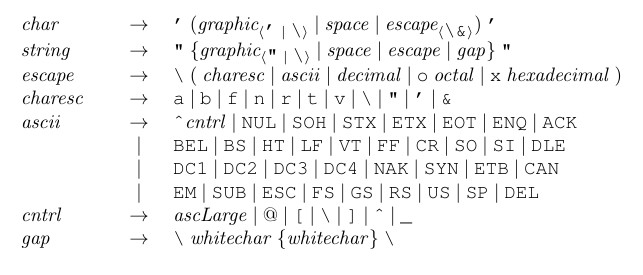
\includegraphics[scale=0.66]{pic-char-string-literals}
\end{figure}

Символьные литералы записываются в одинарных кавычках, а строковые в двойных.
Примеры: \texttt{'a'}, \texttt{"Hello, World!"}.

